\newpage
\section{Použití trezoru}
První nasazení trezoru na akci pořádané Robotárnou \parencite{robotarna} proběhla na příměstském robotickém táboře v srpnu roku 2019.
Jednalo se o první variantu trezoru která kdy spatřila světlo světa \ref{E1-vyvoj}. Tábor trval pět dní a děti dostali první tři dny na stavbu mechaniky a poslední dva dny 
se~programovalo. 

Trezor tehdy sklidil úspěch a tak započal vývoj dalších verzí které už byli specializovanější \ref{E2-vyvoj} \ref{E3-vyvoj} a přidali se i mechanické 
varianty \ref{M1-vyvoj} \ref{M2-vyvoj} \ref{M3-vyvoj}.

\paragraph{Trezor ve volnočasových kurzek robotiky}
Další používání trezoru probíhalo v jednom volnočasovém kurzu robotiky který jsem spoluvedl a účastníci v něm stavěli nejprve tehdy aktuální mechanickou variantu, verzi M2 \ref{M2-vyvoj}.
Protože účastníci kurzu byli vetšinou již docela zkušení, jednalo se u nimi téměř jen o \uv{rozcvičku} kterou měli za několik kroužků hotovou a následovala stavba trezoru E3. 

Bohužel kvůli pandemickým opatřením si ne všichni účastníci stihli trezor postavit a vůbec jsme se nedostali k programování, natož aby jsme si s trezorem zorganizovali nějakou herní akci, 
jak bylo dříve v plánu.

\paragraph{Trpasličí trezor}
Chvíli po té co vznikl trezor M3 \ref{M3-vyvoj} \ref{M3-popis} proběhla první akce s trezorem které nebyla pod taktovkou Robotárny \parencite{robotarna}. Zároveň to byla také 
první akce na které se trezor nestavěl a jen se využíval.

Protože na akci byly menší děti, byl trezor místo klasické číselné stupnice  vybaven obrázkovým kódem, jak je vidět na obrázku \obr{fig:M3-trpaslici}.

Toto však byla poslední akce která se stihla uskutečnit před započetím pandemických opatření.

\begin{figure}[htbp]
    \centering
    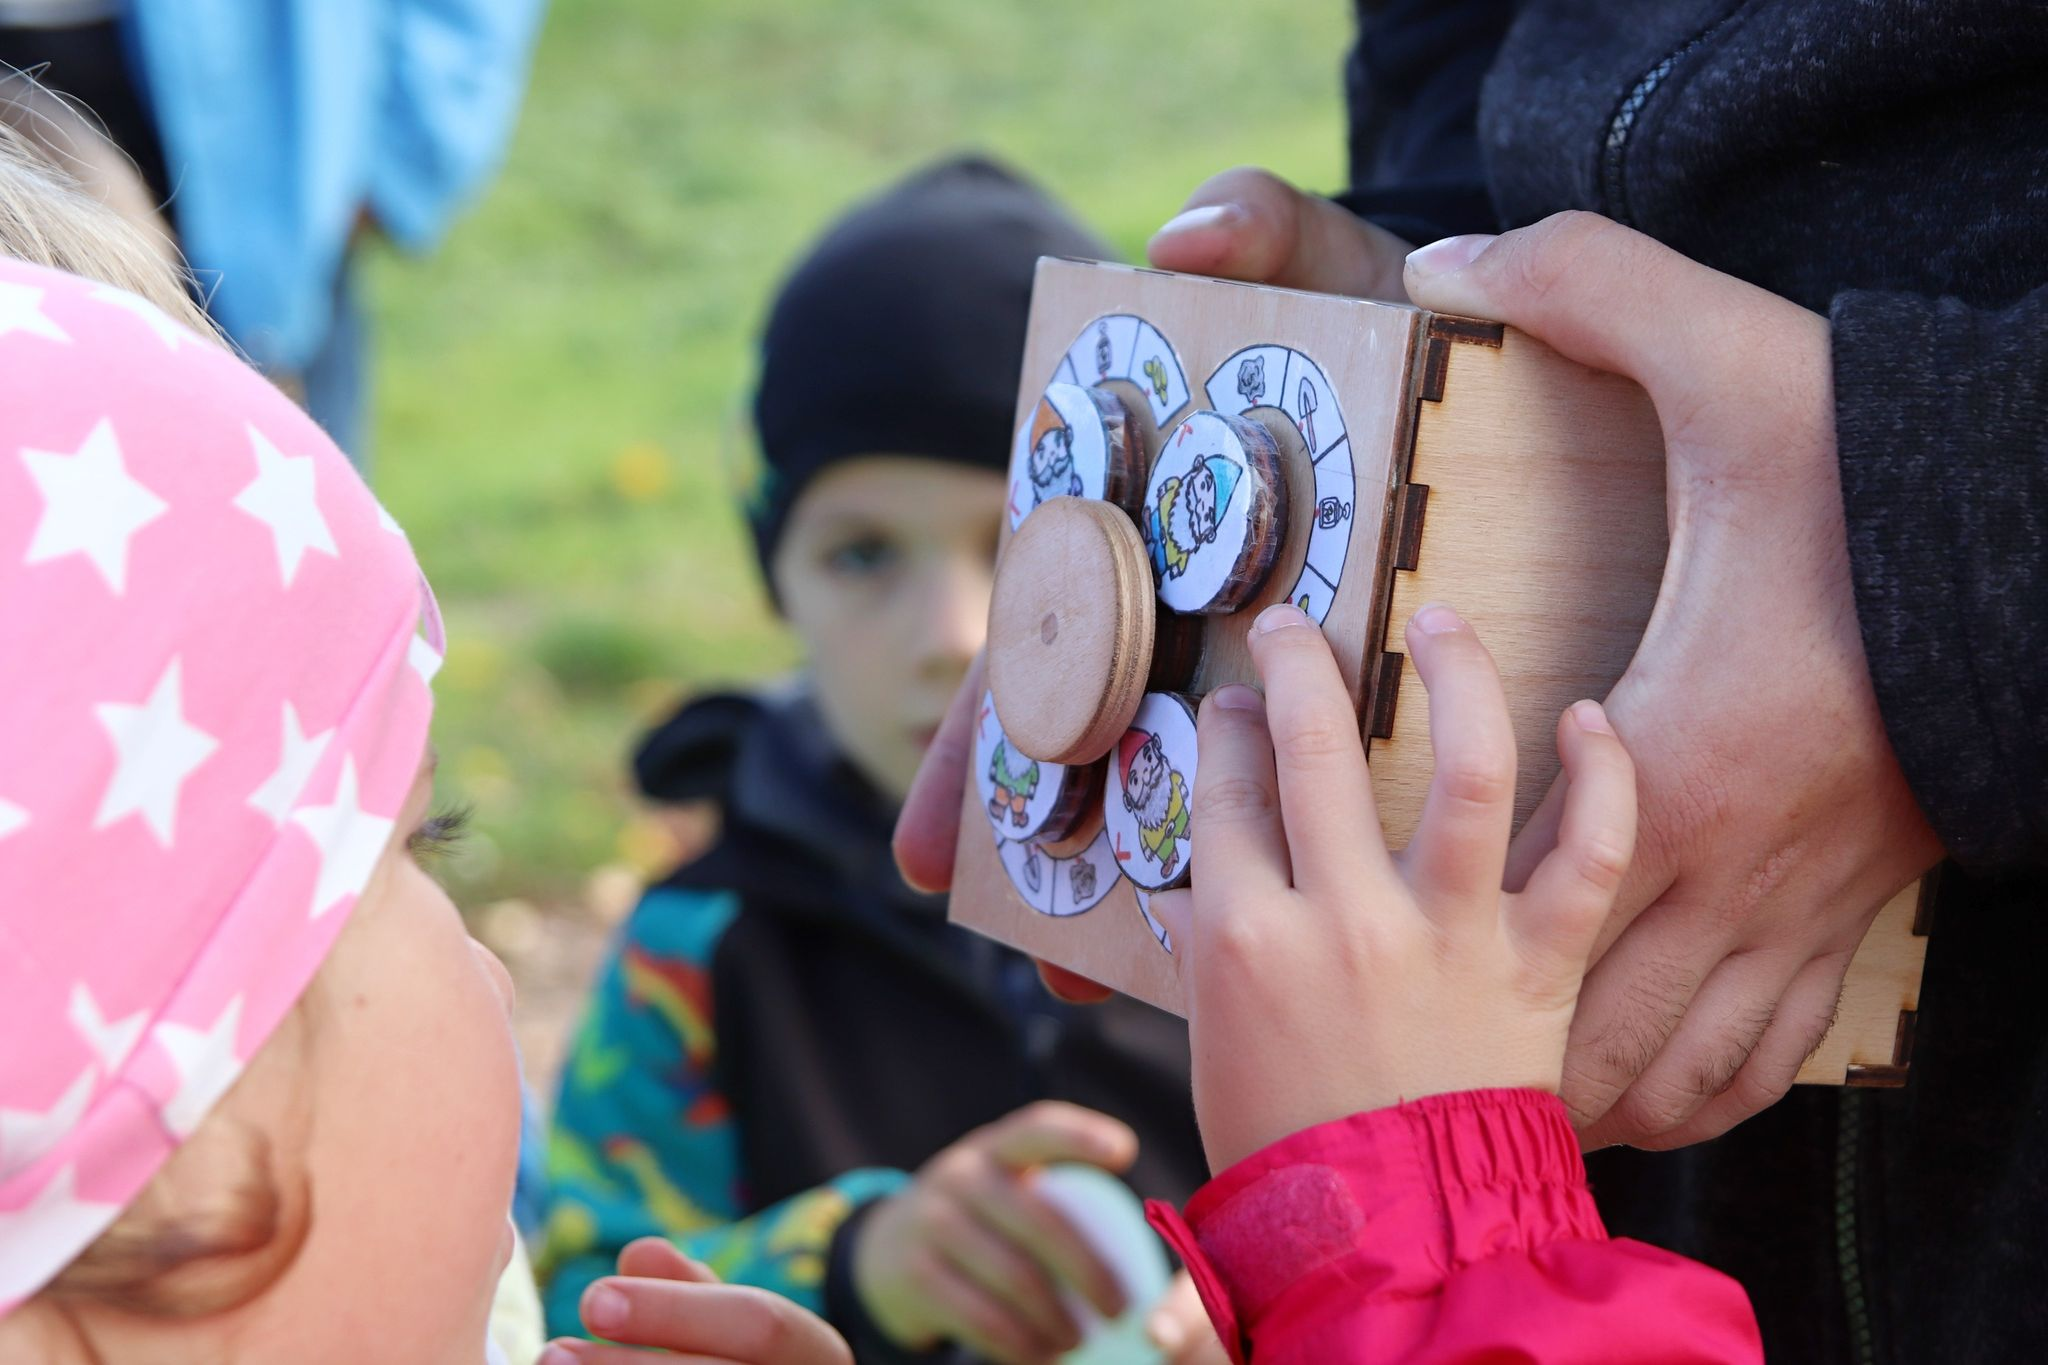
\includegraphics[width=\textwidth]{kapitoly/obrazky/M3/trpaslici.png}
    \caption{Trpasličí trezor}
    \label{fig:M3-trpaslici}
\end{figure}

%todo další akce nikdy moc nebyli v plánu, prostě se už počítalo s lockdownem takže se ani nic nevymýšlelo
%todo jediné co mě ještě napadá je jedna akce kterou měl pod taktovkou Jirka musím mu zavolat (píšu to ve tři ráno takže pokud to čteš tak je to spíš poznámka pro mě abych si na to ráno vzpomněl)